\chapter{Конструкторский раздел}
\label{cha:design}
\textbf{Требования к вводу:}
\begin{enumerate}[1)]
	\item на вход подаются 2 строки;
	\item прописные и строчные буквы считаются разными символами.
\end{enumerate}
\textbf{Требования к программе:} две пустые строки являются корректным вводом.
\section{Схемы алгоритмов}
На рисунках 2.1-2.4 представлены схемы алгоритмов поиска расстояния Левенштейна и Дамерау-Левенштейна.\\
\label{sec:schemes}
\begin{figure}[H]
	\centering
	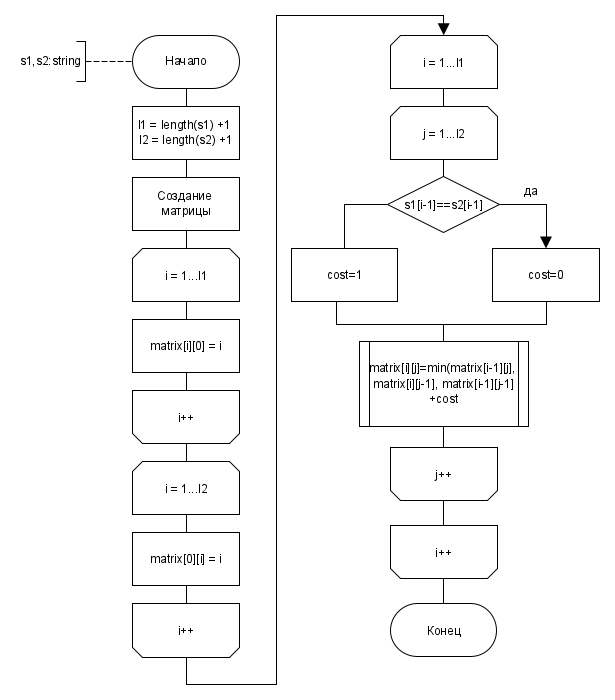
\includegraphics[width=0.6\linewidth]{src/Levenstein_m}
	\caption{Схема матричного алгоритма поиска расстояния Левенштейна}
	\label{fig:levensteinm}
\end{figure}
\begin{figure}[H]
	\centering
	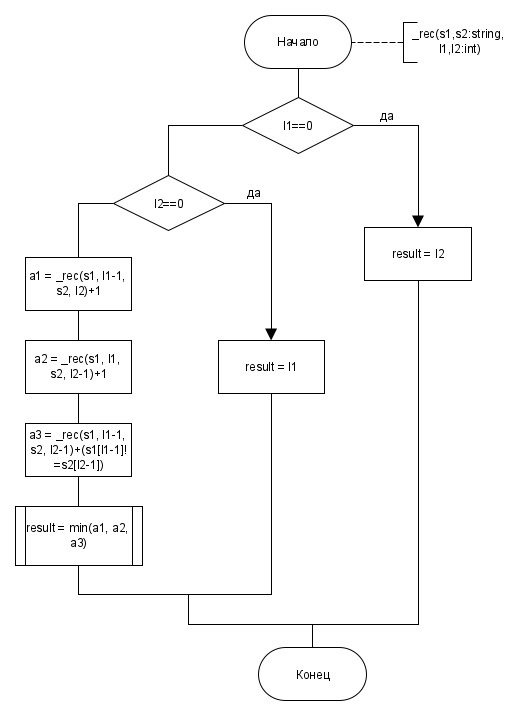
\includegraphics[width=0.7\linewidth]{src/Levenstein_r}
	\caption{Схема рекурсивного алгоритма поиска расстояния Левенштейна}
	\label{fig:levensteinr}
\end{figure}
\begin{figure}
	\centering
	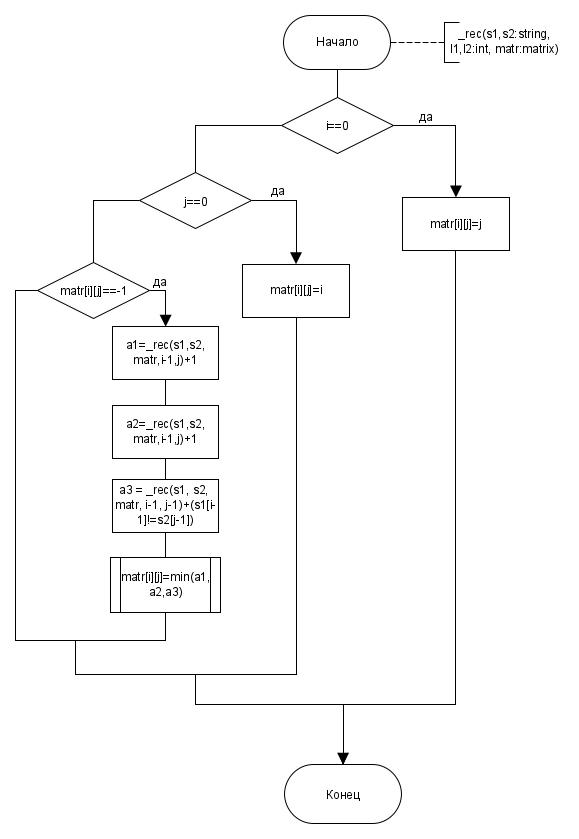
\includegraphics[width=0.8\linewidth]{src/Levenstein_rm}
	\caption{Схема матрично-рекурсивного алгоритма поиска расстояния Левенштейна}
	\label{fig:levensteinrm}
\end{figure}
Отличием матрично-рекурсивного алгоритма поиска расстояния Левенштейна от рекурсивного является сохранение результатов в матрицу, благодаря чему нет необходимости повторно пересчитывать значения функций.
\begin{figure}
	\centering
	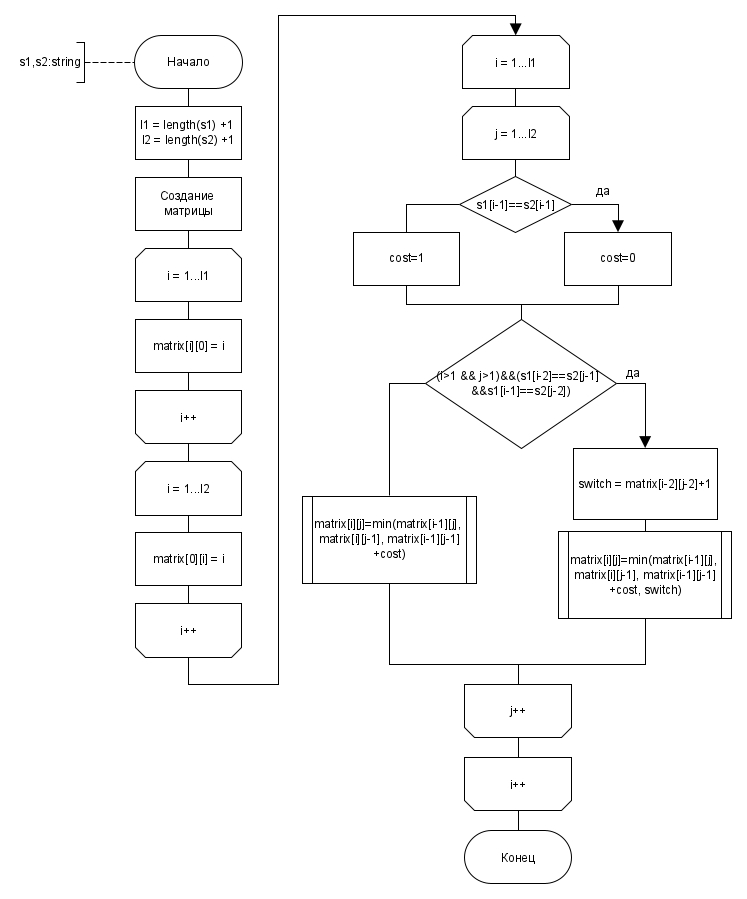
\includegraphics[width=0.8\linewidth]{src/Damerau_m}
	\caption{Схема матричного алгоритма поиска расстояния Дамерау-Левенштейна}
	\label{fig:dameraum}
\end{figure}
